\section{Clustering}

The goal of this section is to introduce another unsupervised learning task: \important{clustering}. We will also introduce K-means clustering and the Fisher Linear Discriminant Analysis, which combines notions of clustering and of dimensionality reduction.

\subsection{Clustering: Another unsupervised learning task}
The goal of this task is: given some input data, we want to answer the question 
\begin{center}
    '\textit{can we identify groups, without performing any data transformation?}'
\end{center}
This operation is called \important{clustering}.
\begin{parag}{A simple clustering algorithm}
    Let us now define the $K$-means clustering:
	\begin{itemize}
	    \item Given a set of input samples, group the samples into $K$ clusters
	    \item $K$ is a hyper-parameter, assumed to be known/given
	    \item In the toy example below, each data sample is a point in 2D.
	\end{itemize}
	\begin{center}
	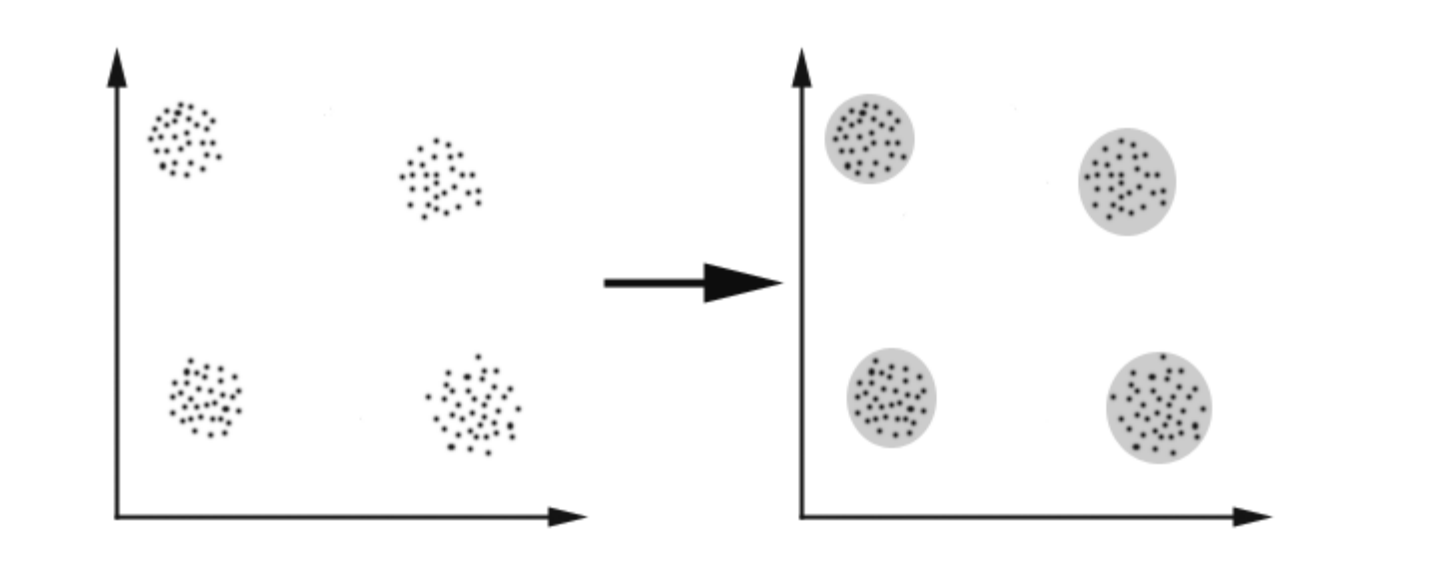
\includegraphics[scale=0.2]{screenshots/2026-05-11.png}
	\end{center}
	The goal is therefore to have the distance between the points \important{within} a cluster being small and the distance \important{across} cluster being large. The distance between clusters can be encoded via distances to cluster centers $\left\{\mu_1, \ldots, \mu_k\right\}$
\end{parag}
\begin{parag}{Algorithm}
    The algorithm in order to compute the $K$ clusters is described below:
	\begin{enumerate}
	    \item Initialize $\left\{\mu_1, \ldots, \mu_k\right\}$ (e.g., randomly)
	    \item While not converged 
			\begin{enumerate}
			    \item Assign each point $x_i$ to the nearest center $\mu_k$ 
					\begin{itemize}
					    \item For each point $x_i$, compute the Euclidean distance to every center $\left\{\mu_1, \ldots, \mu_k\right\}$
					    \item Find the smallest distance
					    \item The point is said to be assigned to the corresponding cluster (not that each point is assigned to a single cluster)
					\end{itemize}
				\item Update each center $\mu_k$ based on the points assigned to it 
					\begin{itemize}
					    \item Recompute each center $\mu_k$ as the mean of the points that were assigned to it
					\end{itemize}
			\end{enumerate}
	\end{enumerate}
\end{parag}
\begin{parag}{More details}
    In the second step, as the algorithm iteratively updates the cluster assignment for each point and the clusters centers, we need to eventually stop iterating. This could be done using an hyper-parameter, we give as input to our algorithm a fixed number of iterations. However this is not ideal as it can lead to either a too big number of iterations or too small which would lead to bad results. As way to know whether or not we are far from the '\textit{local optimal solution}' is to check the difference between the previous center location and the current. We could set a $\delta$ such that while the distance between the $k$ and the $k-1$ iterations is $> \delta$ we continue. However to do so we need to be sure that the algorithm is guaranteed to converge to a stable solution, here it is the case.
\end{parag}
\begin{framedremark}
An important thing to know is that the algorithm will always converges, but it doesn't always converge to the best (desired) solution (this is why I put the optimal solution inside '' before).
\end{framedremark}

\begin{parag}{K-means clustering: Properties}
    In conclusion we have that:
	\begin{itemize}
		\item \textbf{Pros}: It is a simple algorithm that is always guaranteed to converge
		\item \textbf{Cons}: It does not always converge to the best solution
	\end{itemize}
	In order to counter attack this cons above, we could run the algorithm several time with different initialization and, 
	\begin{itemize}
	    \item For each solution, sum the distances of each point to its assigned cluster
	    \item Choose the solution with the smallest sum
	\end{itemize}
	To continues our pros/cons:
	\begin{itemize}
	    \item \textbf{Pros}: Returns exactly $K$ clusters
	    \item \textbf{Cons}: Some clusters might be empty (no samples assigned)
	    \item \textbf{Cons}: Requires the user to determine $K$
	\end{itemize}
	\begin{subparag}{Remark}
	    And as this is unsupervised learning, cross-validation is not an option
	\end{subparag}
	But here we can use the same technique as above (in order to determine $K$), 
	\begin{itemize}
	    \item Run the algorithm with different values of $K$
	    \item For each solution, sum the distances of each point to its assigned cluster
	    \item Plot the resulting curve
	\end{itemize}
	\begin{center}
	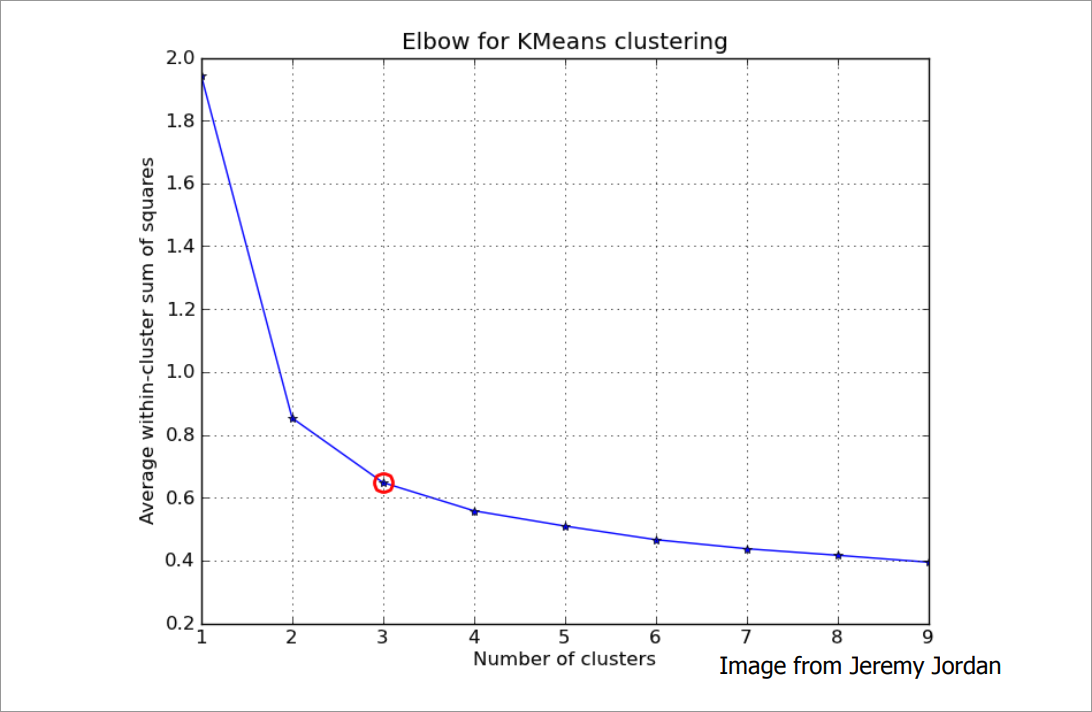
\includegraphics[scale=0.2]{screenshots/2026-05-11_1.png}
	\end{center}
	And as you could have guessed the average within-cluster distance typically decreases towards zero.
	
\end{parag}

\begin{parag}{Other Properties}
    As we don't have any annotations, it requires human analysis to provide a semantic meaning to the clusters. However if annotations are available, they can be sued to label each cluster, e.g., with a corresponding category label. 
	\begin{itemize}
	    \item For each cluster, find the number of samples of each category
	    \item Assign the cluster category with the largest number of samples
	\end{itemize}
	Another property is the \important{euclidean distance}: this distance works well for data with homogeneous dimensions, meaning we don't have spike to some random dimensions. However in practice this is not always the case 
	\begin{itemize}
	    \item Different data dimensions can have completely different magnitudes
	    \item They can encode completely different types of information
	\end{itemize}
	What this implies is that large values will dominate other part of the data point. A solution to this '\textit{problem}' (this isn't really a problem in essence, it is maybe a property that we don't want to have) can be solved using normalization and/or different distance function.
\end{parag}


\paragraph{Clustering and dimensionality reduction}%
\label{par:Clustering and dimensionality reduction}

The dimensionality reduction algorithms we saw last week were unsupervised and thus may not preserve category information. For instance
\begin{center}
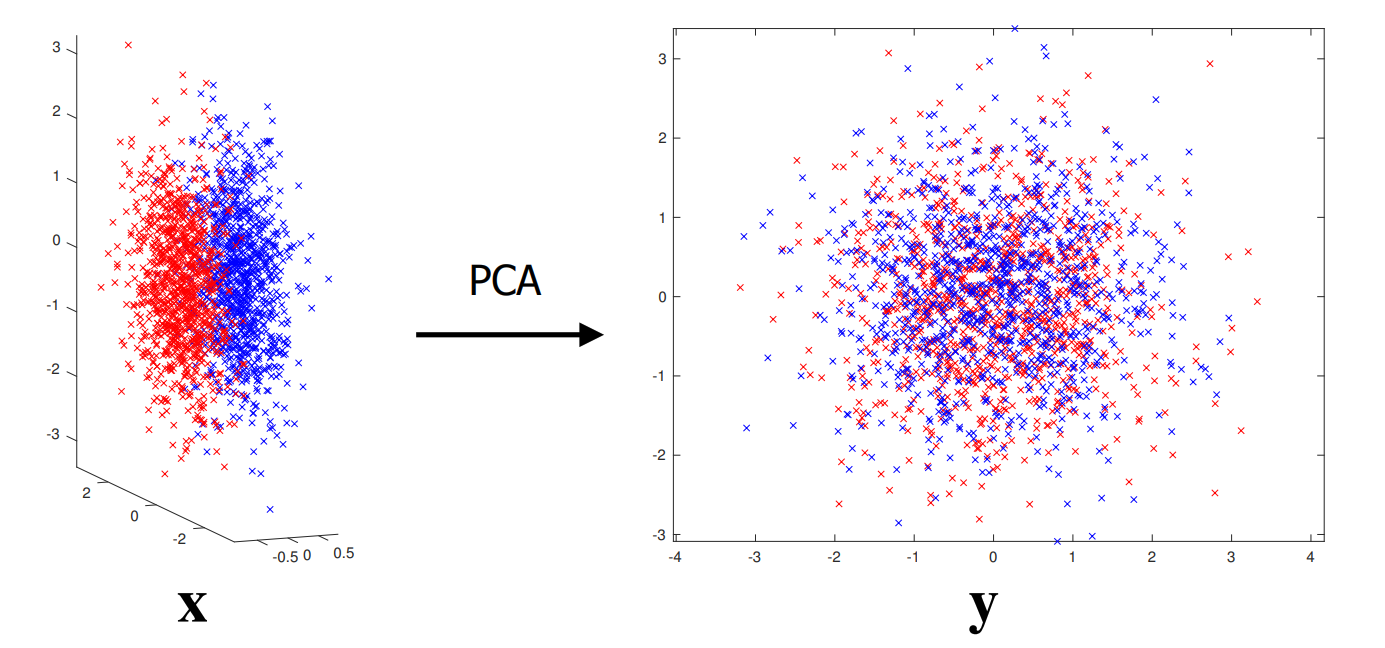
\includegraphics[scale=0.3]{screenshots/2026-05-12.png}
\end{center}
\begin{framedremark}
	Categories are not known, when doing $K$-means nor when doing PCA. The goal or the hope of clustering as we have seen before was to '\textit{guess}' those categories by making clusters of data. So it would feel like supervised learning but it really isn't. When training/running our algorithm we don't have any ground truth label to refer to. \\
	$ $\\
	I feel like the image above is a bit misleading. When doing PCA, we wouldn't have any colour. Therefore the goal is to be able to find those cluster in the new dimension with the use of the class label.
\end{framedremark}

What could have been done is to use the actual information that we are missing when doing the dimension reduction: the \important{label}. The goal would be to use those label during the dimensionality reduction to encourage clustering in the low-dimensional space.

\begin{parag}{Fisher Linear Discriminant Analysis (LDA)}
	As we have said before the goal that we would like to obtain is 
	\begin{itemize}
	    \item The samples from the same class to be clustered
	    \item The different classes to be separated
	\end{itemize}

	\begin{center}
	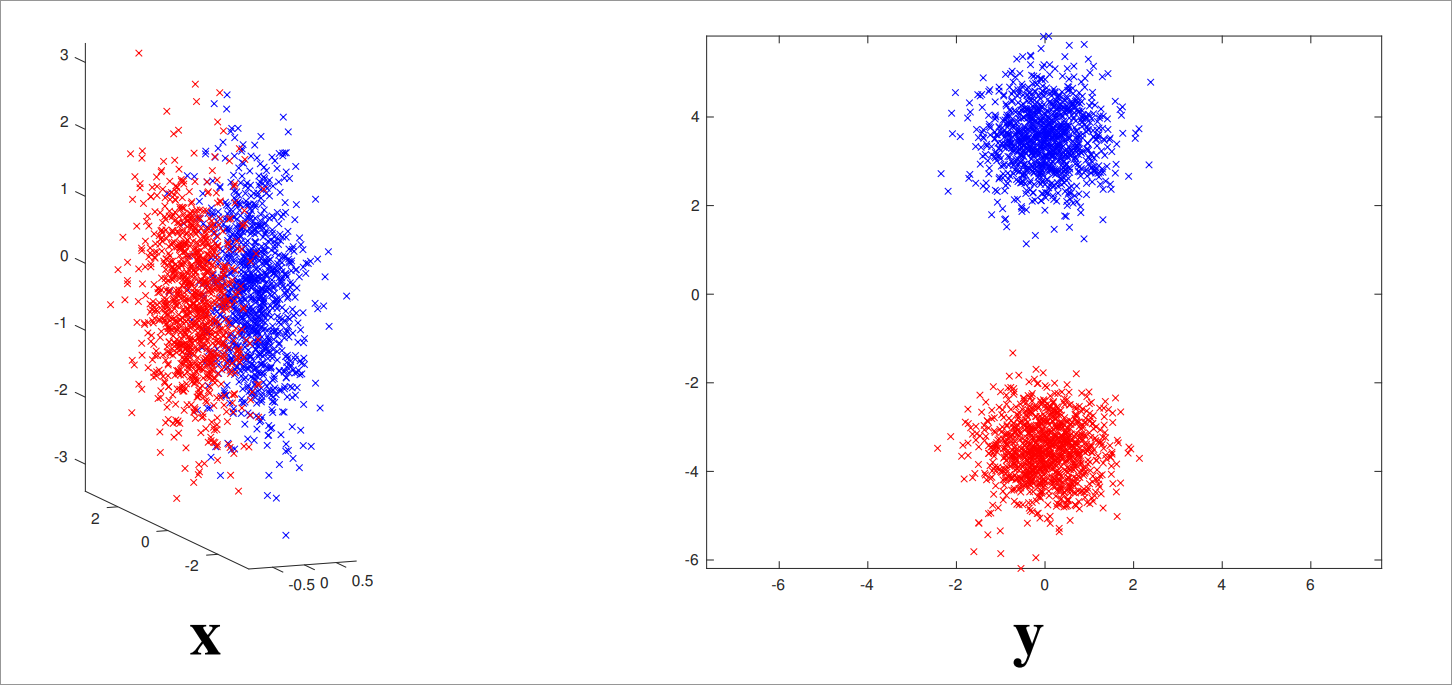
\includegraphics[scale=0.3]{screenshots/2026-05-12_1.png}
	\end{center}	
	Therefore now we are back to supervised learning (even though the supervision is not given for the $\left\{y_i\right\}$ directly but via the class labels).
	
\end{parag}


\begin{parag}{Clustering the sample from the same class}
    Mathematically, this means that we want a low variance within each class after projection.\\
	$ $\\
	For a 1D projection, encoded via a vector $w_{\left(1\right)}$, and $C$ classes, this can be expressed as aiming to minimize 
	\begin{align*} 
		E_W\left(w_{\left(1\right)}\right) = \sum_{c= 1}^{C}\sum_{i \in c} \left(y_i - \nu_c\right)^2
	\end{align*}
	Where $\nu_c$ is the mean of the samples in class $c$ after projection, and $i \in \nu_c$ indicates that sample $i$ belongs to class $c$.
	\begin{subparag}{Remark}
	    Note that both $y_i$ and $\nu_c$ depend on $W_{\left(1\right)}$
	\end{subparag}
	As in the PCA case, the variance after projection is equal to the projection of the covariance matrix. This lets us rewrite the previous objective function as 
	\begin{align*} 
		E_{W}\left(w_{\left(1\right)}\right) = w_{\left(1\right)}^{T}S_Ww_{\left(1\right)}
	\end{align*}
	Where 
	\begin{align*} 
		S_W = \sum_{c= 1}^{C}\sum_{i \in c} \left(x_i - \mu_c\right)\left(x_i - \mu_c\right)^{T}
	\end{align*}
	With $\mu_c$ the mean of the data in class $c$ \important{before} projection. $S_W$ is referred to as the \important{within} class scatter matrix.
\end{parag}

\begin{parag}{Separating the different classes}
    In addition to clustering the samples according to the classes, we want to separate the different clusters. This can be achieved by pushing the means of the clusters away from each other. Mathematically, this can be expressed as maximizing 
	\begin{align*} 
		W_B\left(w_{\left(1\right)}\right) = \sum_{c= 1}^{C}N_c \left(\nu_c - \overline{y}\right)^2
	\end{align*}
	Where $\nu_c$ is defined as before, $\overline{y}$ is the mean of all samples after projection, and $N_c$ is the number of samples in class $c$. Again following the same reasoning as before, this can be re-written as 
	\begin{align*} 
		E_B\left(w_{\left(1\right)}\right) = w_{\left(1\right)}^{T}S_Bw_{\left(1\right)}
	\end{align*}
	Where 
	\begin{align*} 
		S_B = \sum_{c= 1}^{C}N_C\left(\mu_c - \overline{x}\right)\left(\mu_c - \overline{x}\right)^{T}
	\end{align*}
	With $\overline{x}$ the mean of all samples and $\left\{\mu_c\right\}$ the class specific means.\\
	$ $\\
	$S_B$ is referred to as the \important{between-class} scatter matrix
\end{parag}


\begin{parag}{Fisher LDA}
    Altogether, we want to 
	\begin{itemize}
	    \item minimize $E_W\left(w_{\left(1\right)}\right)$
	    \item maximize $E_B\left(w_{\left(1\right)}\right)$
	\end{itemize}
	This can be achieved by maximizing 
	\begin{align*} 
		J\left(w_{\left(1\right)}\right) = \frac{E_B\left(w_{\left(1\right)}\right)}{E_W\left(w_{\left(1\right)}\right)} = \frac{w_{\left(1\right)}^{T}S_Bw_{\left(1\right)}}{w_{\left(1\right)}^{T}S_Ww_{\left(1\right)}}
	\end{align*}
	And we can easily see that the previous objective function is invariant to scaling 
	\begin{align*} 
		J\left(\alpha w_{\left(1\right)}\right) =  J\left(w_{\left(1\right)}\right) \mathspace \forall \alpha \in \mathbb{R}
	\end{align*}
	We can therefore fix the scale by constraining $w_{\left(1\right)}$ to be such that 
	\begin{align*} 
		w_{\left(1\right)}^{T}S_Ww_{\left(1\right)} = 1
	\end{align*}
	This yields the Fisher LDA formulation 
	\begin{align*} 
		\max_{w_{\left(1\right)}}w_{\left(1\right)}^{T}S_Bw_{\left(1\right)}\\
		\text{s.t. } w_{\left(1\right)}^{T}S_W w_{\left(1\right)} = 1
	\end{align*}
	And as before, we rely on the Langragian, written as 
	\begin{align*} 
		\mathcal{L}\left(w_{\left(1\right)}, \lambda_1\right) = w_{\left(1\right)}^{T}S_Bw_{\left(1\right)} + \lambda\left(1 - w_{\left(1\right)}^{T}S_Ww_{\left(1\right)}\right)
	\end{align*}
	Zeroing out the gradient of $\mathcal{L}$ w.r.t. $w_{\left(1\right)}$ yields 
	\begin{align*} 
		S_B w_{\left(1\right)} =  \lambda_1 S_W W_{\left(1\right)}
	\end{align*}
	this implies that $w_{\left(1\right)}$ must be the solution to a generalized eigenvector problem.
	\begin{subparag}{Remark}
	    By left multiplying both side by $w_{\left(1\right)}^{T}$ and dividing by $w_{\left(1\right)}^{T}S_Ww_{\left(1\right)}$ tells us that $w_{\left(1\right)}$ should be eigenvector with largest eigenvalue
	\end{subparag}
\end{parag}


\begin{parag}{Dealing with $d > 1$}
    To project the data to more than a single dimension, we can follow a recursive strategy similar to the PCA one. Ultimately, this consists of taking the $d$ eigenvector with the largest eigenvalues.\\
	$ $\\
	Note that it can be shown that $S_B$ has rank at most $C - 1$ and therefore, we can project data only to at most $C - 1$ dimensions (as the remaining eigenvalues will all be $0$ and thus carry no information)
	
\end{parag}





\begin{parag}{Compactness}
    $K$-means clustering (and Fisher LDA) exploit the notion of \important{compactness} of clusters. The question now is: what would happen if the data is not compact, for instance 
	\begin{center}
	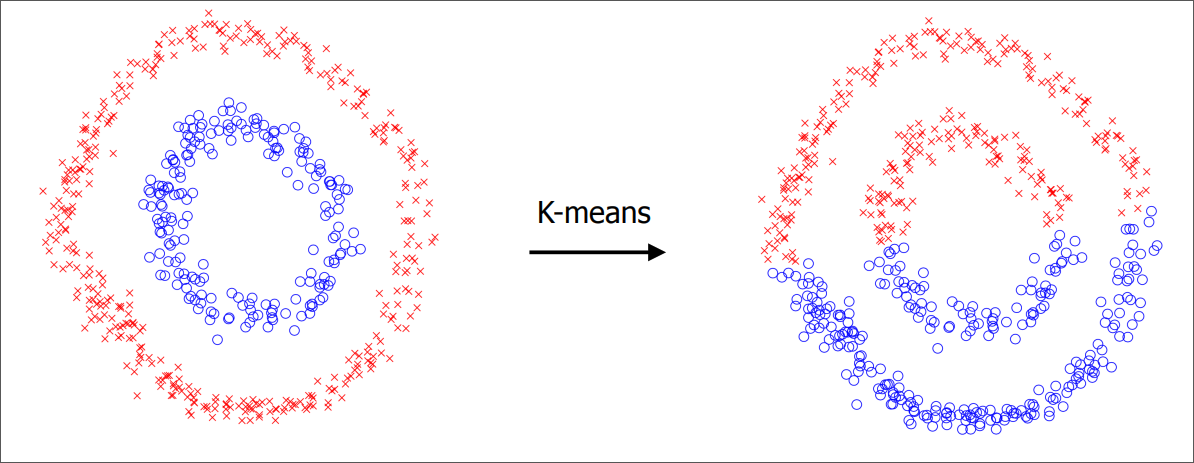
\includegraphics[scale=0.2]{screenshots/2026-05-12_2.png}
	\end{center}
	Even in this case, we are still able to clearly identify the two '\textit{true}' clusters.\\
	$ $\\
	But before that let us concentrate ourself on the image on the left. Here, the two clusters we observe arise from the connectivity of the points. We would like to have a method that works well for those type of relation.
\end{parag}

\begin{parag}{Spectral clustering: Graph-based connectivity}
	The idea now is to group points based on edges in a graph, strong connections indicate points that should be clustered whereas weaker ones suggest that the graph can be cute into pieces/partitions
	\begin{center}
	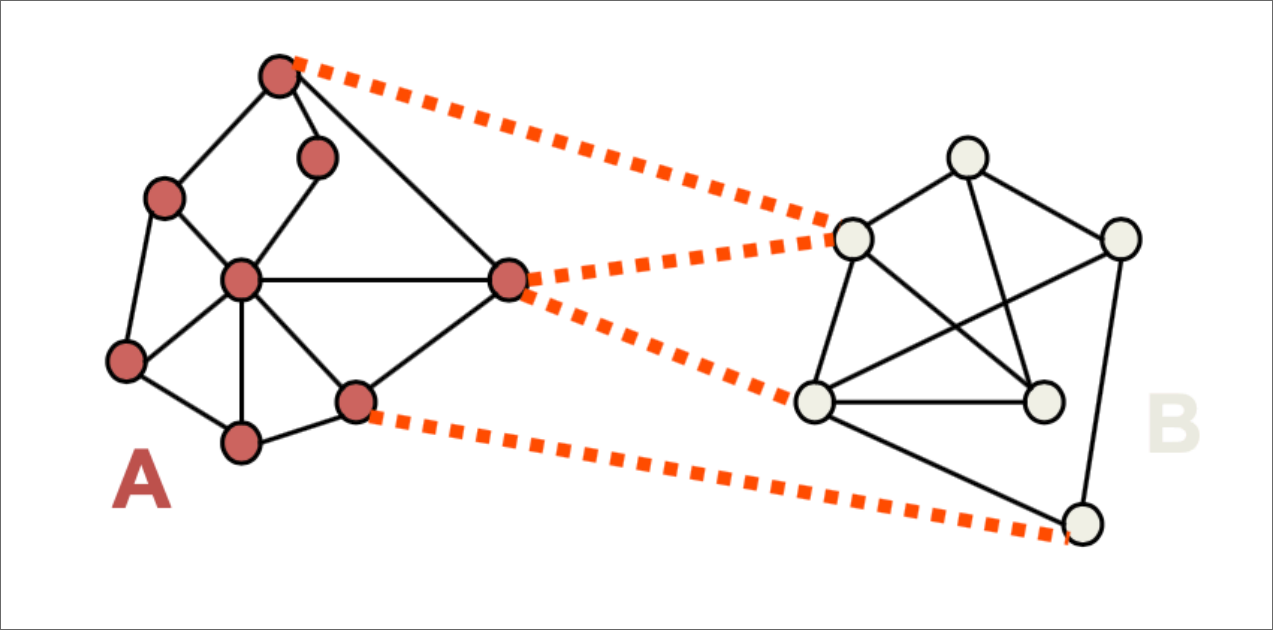
\includegraphics[scale=0.2]{screenshots/2026-05-12_3.png}
	\end{center}
	The question that we have now, is how do we create this graph in the first place. To do so we need to introduce the notion of similarity between the points. For instance we can take the definition below for given point $i$ and $j$
	\begin{align*} 
		W_{ij} = \exp\left(\frac{-\left\|x_i - x_j\right\|^2}{\sigma^2}\right)
	\end{align*}
	Where $\sigma$ is a hyper-parameter. And as you could have guessed, this would lead to a fully connected graph (an edge with a weight $W_{ij}$ for every pair of points). The graph can also be restricted to the $K$-nearest neighbour of each point. Therefore a graph ca equivalently be represented by a similarity matrix $W$.
\end{parag}

\begin{parag}{Graph cut}
    Consider a partition of a graph into two parts $A$ and $B$.
	\begin{center}
	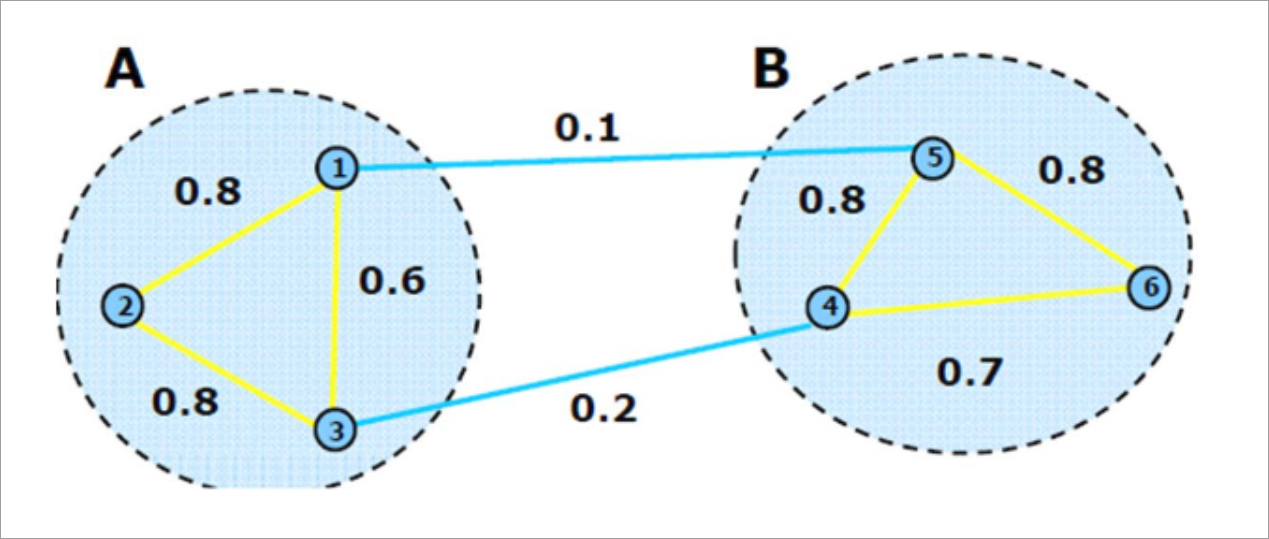
\includegraphics[scale=0.2]{screenshots/2026-05-12_4.png}
	\end{center}
	(vraiment rude le screen si j'ai la force je refais en svg)\\
	$ $\\
	A cost for cut is obtained by summing the weight of the edges that connect the two groups
	\begin{align*} 
		\text{cut}\left(A, B\right) = \sum_{i \in A, j \in B}W_{ij}
	\end{align*}
	In the above example, this would give us $0.3$.\\
	$ $\\
	Intuitively, for clustering, we would like to find partition that minimizes such a cut.
\end{parag}

\begin{parag}{Graph terminology}
	\begin{definition}{degree}
    The degree of a node in the graph is given by 
	\begin{align*} 
		d_i = \sum_{j} W_{ij}
	\end{align*}
    \end{definition}
	\begin{definition}{volume}
	The volume of a set (partition) is given by 
	\begin{align*} 
		\text{vol}\left(A\right) = \sum_{i \in A}d_i
	\end{align*}
	\end{definition}
	\begin{subparag}{Remark}
	    I will still need to check but, here we have that all edge within a graph are counted double whereas crossing edges are counted only once. 
	\end{subparag}
\end{parag}


\begin{parag}{Normalized cut}
    Minimizing the cut might favor imbalanced partitions (e.g., a single point in $A$ and all others in $B$) instead we could use a normalized cut 
	\begin{align*} 
		\text{Ncut}\left(A, B\right) = \frac{\text{cut}\left(A, B\right)}{\text{Vol}\left(A\right)} + \frac{\text{cut}\left(A, B\right)}{\text{Vol}\left(B\right)}
	\end{align*}
\end{parag}


\begin{parag}{Transformed formulation}
    Finding the partition that minimizes the normalized cut is NP hard. A way to counter this is to re-write it as an optimization problem 
	\begin{align*} 
		\min_y \frac{y^{T}\left(D - W\right)y}{y^{T}Dy}\\
		\text{s.t. } y^{T}D I = 0\\
		y_i \in \left\{1, -b\right\}, \mathspace \forall 1 \leq i \leq N
	\end{align*}
	Where 
	\begin{itemize}
	    \item $W \in \mathbb{R}^{N \times N}$ is the similarity matrix between all pairs of points
	    \item $D in \mathbb{R}^{N \times N}$ is the diagonal matrix degree matrix, with $D_{ii} = d_i$
	    \item $y$ indicates to which partition each point belongs
	\end{itemize}
	However even with that, this remains an NP hard problem. But we are not done! We can again relax this problem as 
	\begin{align*} 
		\min_y y^{T}\left(D - W\right)y \\
		\text{ s.t. }y^{T}Dy = 1
	\end{align*}
	And using the Lagrangian, the solution can be expressed as a generalized eigenvalue problem 
	\begin{align*} 
		\left(D - W\right)y = \lambda Dy
	\end{align*}

	
	\begin{subparag}{Note}
	    $\left(D - W\right)$ is referred to as the graph Laplacian.
	\end{subparag}
	The question now is \important{which eigenvector}, the eigenvector with the smallest eigenvalue is a vector of all $1$, its eigenvalue is $0$. Therefore we cannot take this one, we need to take the second one.
	\begin{itemize}
		\item ideally, a positive value in this vector indicates that the corresponding point belongs to one partition, and a negative value to the other
		\item Because of the relaxation, this is not so ideal; one then needs to threshold the values (e.g., by taking the median value as threshold for balanced data)
	\end{itemize}
	\begin{center}
	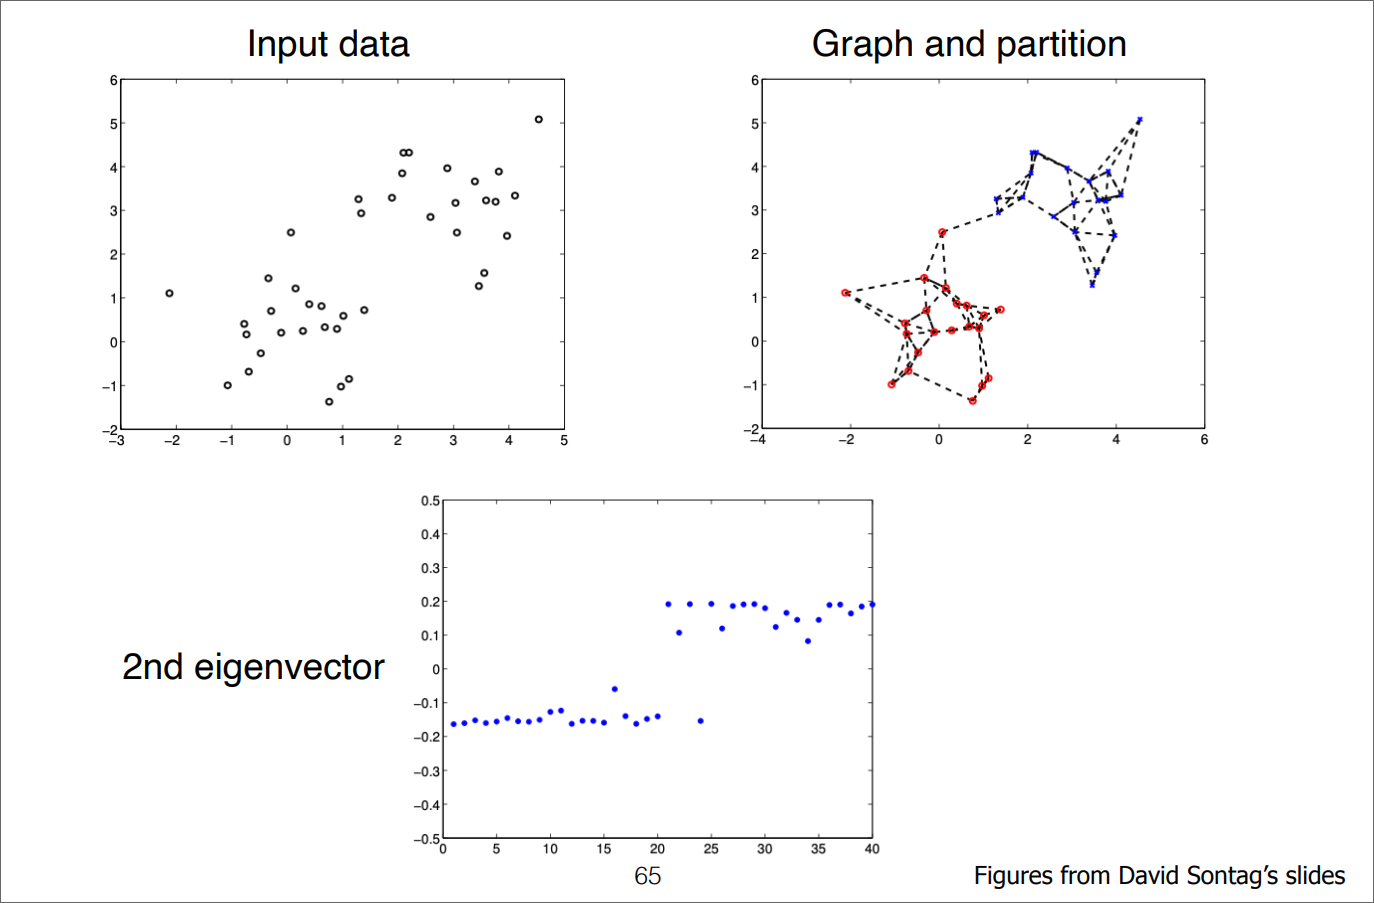
\includegraphics[scale=0.3]{screenshots/2026-05-12_5.png}
	\end{center}
\end{parag}

\begin{parag}{$K$-way partition}
    To obtain more than 2 clusters, one can either 
	\begin{itemize}
	    \item Recursively apply the 2-way partitioning algorithm (Not efficient unstable)
	    \item Use multiple (i.e., $K$) eigenvectors 
			\begin{itemize}
			\item Each point is represented as a $K$-dimensional vector
			\item Apply $K$-means clustering to the resulting $N$ vectors
			\item Interpretation: Dimensionality reduction followed by $K$-means
			\end{itemize}
	\end{itemize}
	\begin{center}
	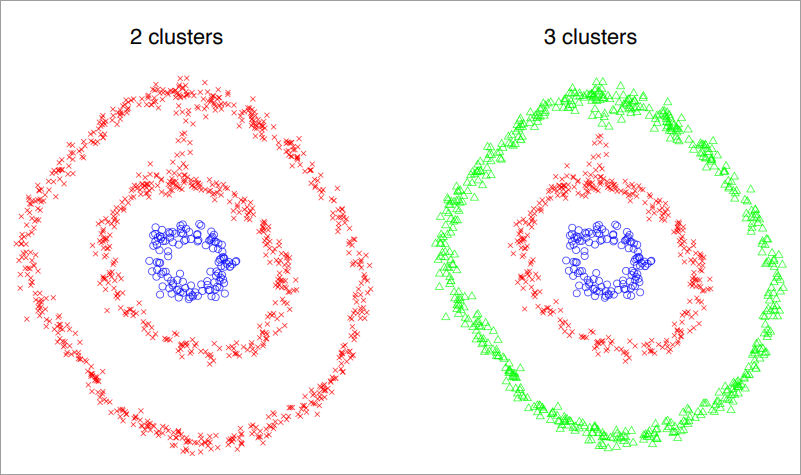
\includegraphics[scale=0.3]{screenshots/2026-05-12_6.png}
	\end{center}
	
\end{parag}









